\subsection{Echo chambers}
In news media, \textit{echo chamber} is a metaphorical description
of a situation in which beliefs are amplified or reinforced by
communication and repetition inside a closed system\cite{echochamwiki,echocham}.\\
We qualitatively investigated the presence of echo chambers in our network.
First of all, our agents have a ``mental  state'', i.e. a vector of preferences: its components represent the amount of interest toward a certain topic.\\
 News have the same dimension of \textit{mental state vector} (MSVD) in order to establish a ``matching'' between news' topics and users' preferences.
 Mental state is highly involved in news' dynamics and network topology.\footnote{See section~\nameref{introduction} for more details on the previous work.}\\
 In the images below, for MSVD=3,5,7, we extracted main clusters from our network.
 Memory length is twelve for all the simulations.\\
 \textit{Modularity} is a measure for detecting community structure in graphs\cite{modulwiki}.
 To provide a comparison, nodes were painted with modularity class and the most recent news in memory.
 In case of news' homogeneity inside a single cluster, we are observing an echo chamber.\\
We can notice that number of clusters equals MSVD basically.
News' situation is more heterogenous: altough some clusters still exist, there is not a clear separation among users with different news.


\begin{figure}
  \centering
  \begin{subfigure}[t]{0.25\textwidth}
    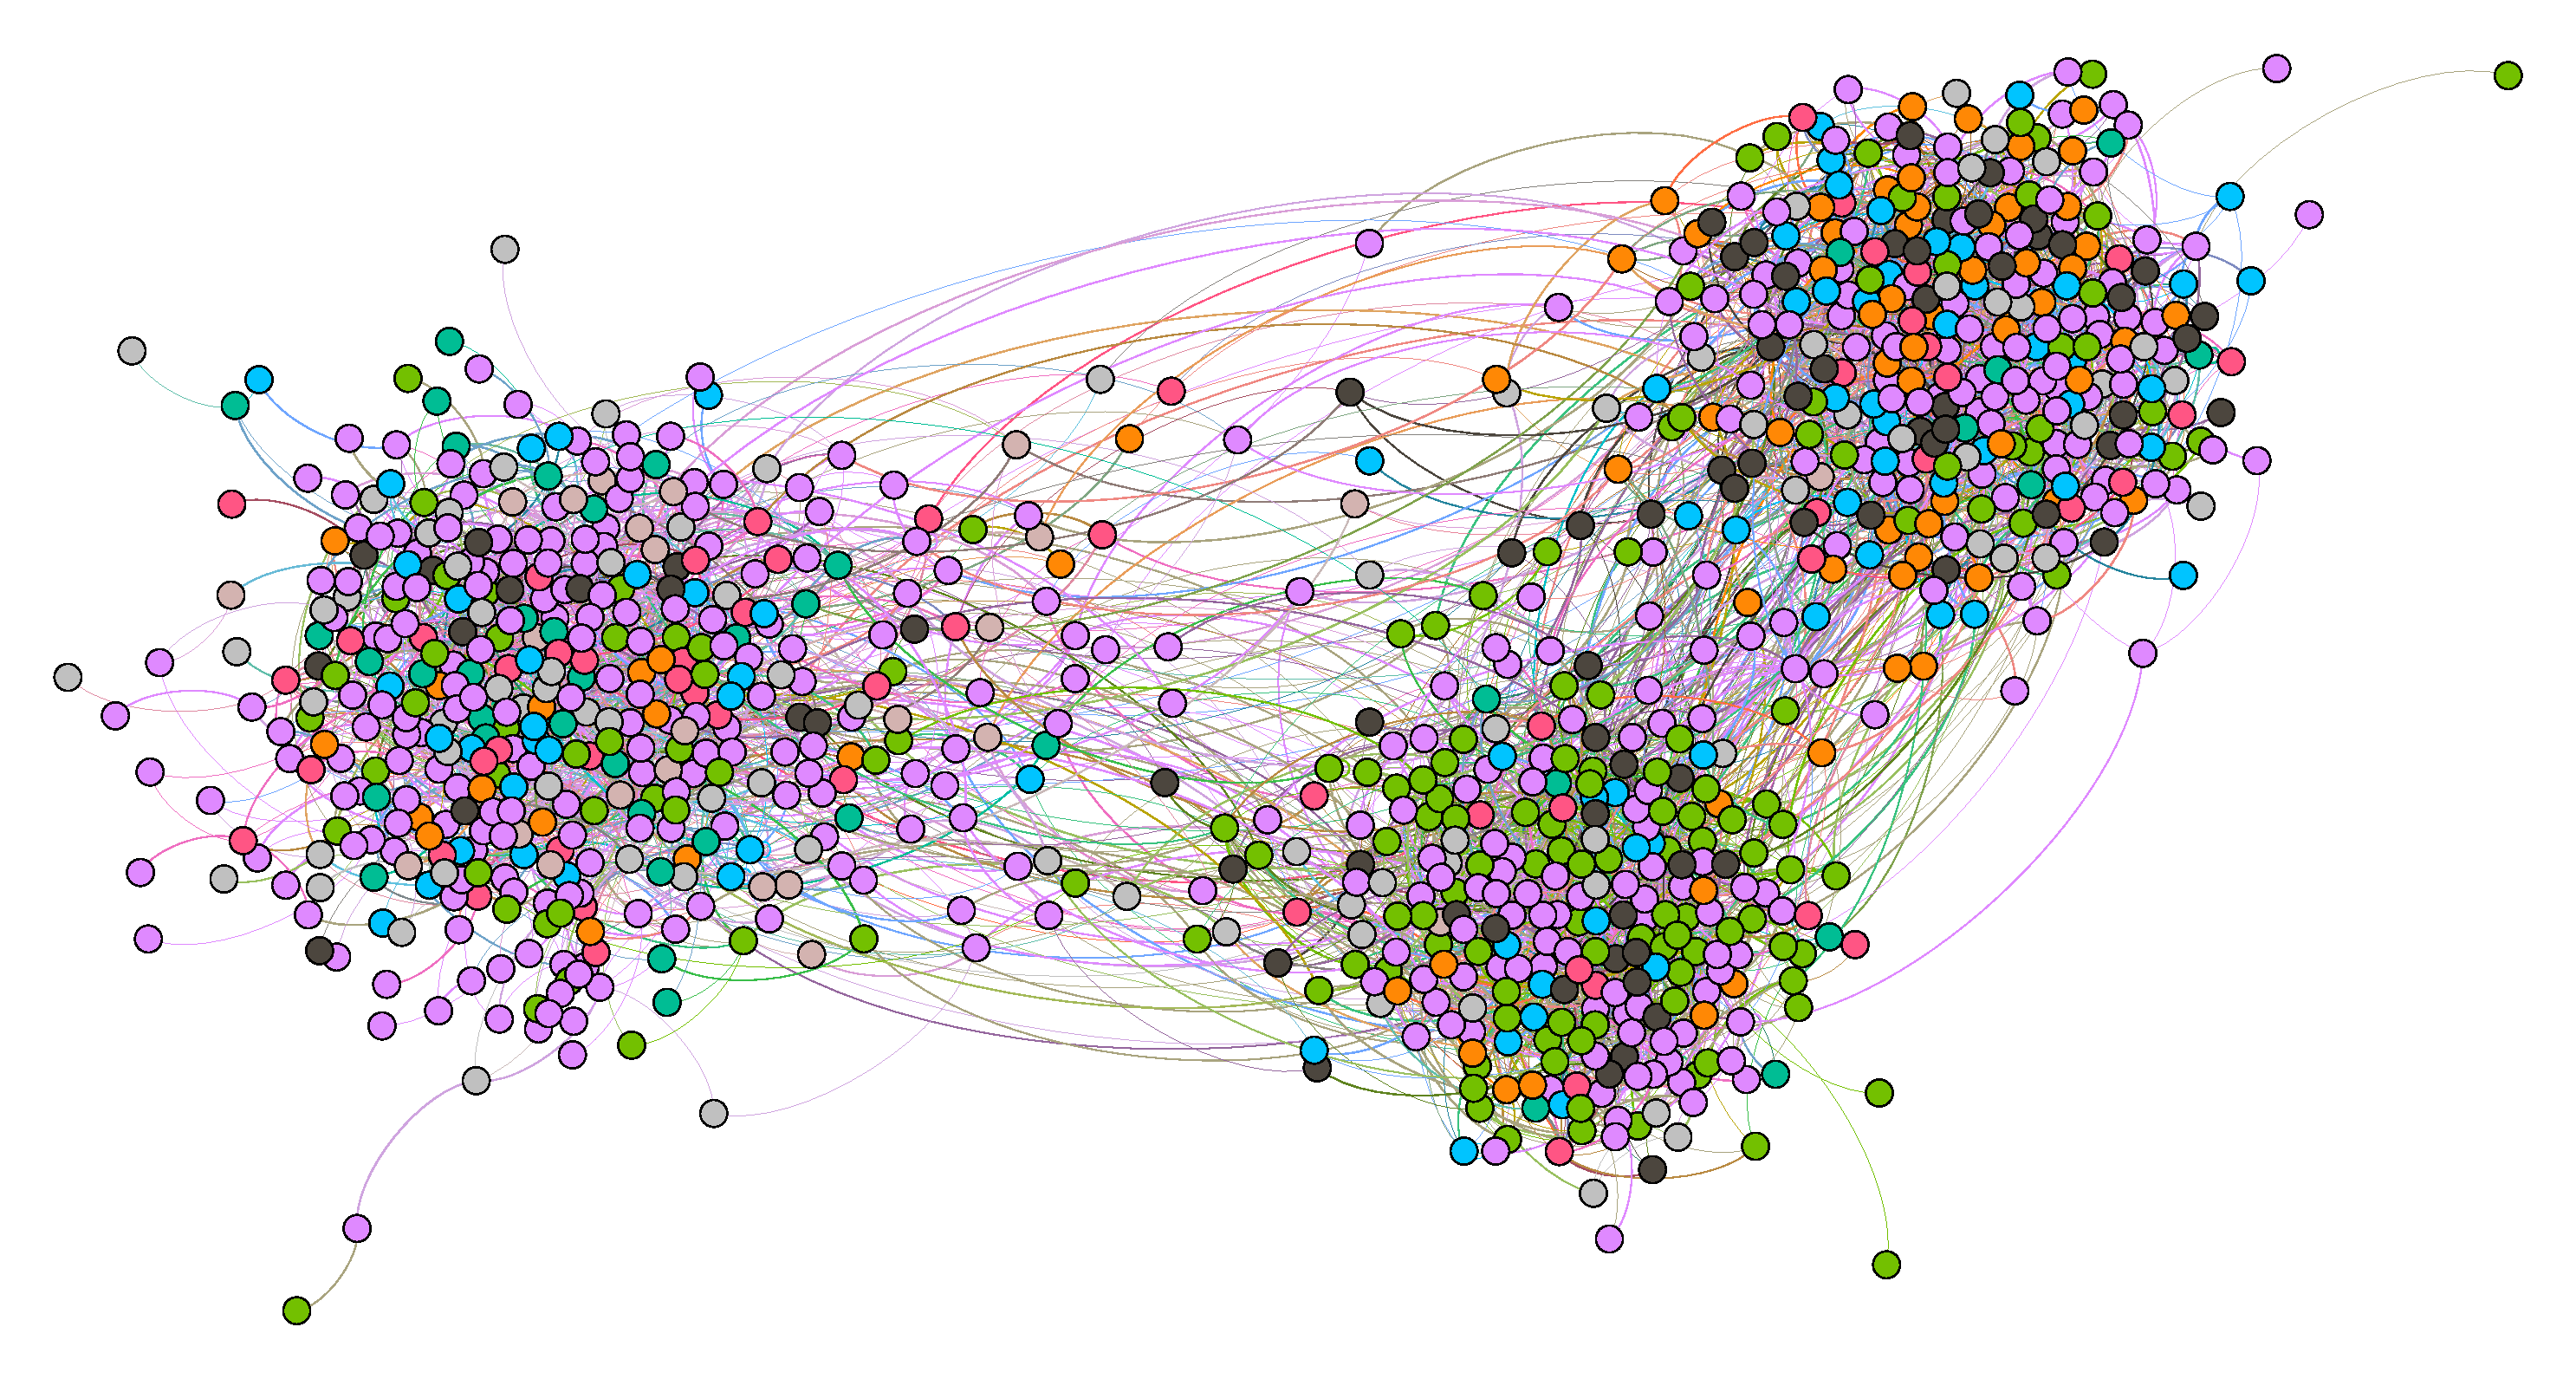
\includegraphics[width=\textwidth]{img/dim3_mod.pdf}
    \caption{}
    \label{fig:bubble3mod}
  \end{subfigure}
  ~
  \begin{subfigure}[t]{0.35\textwidth}
    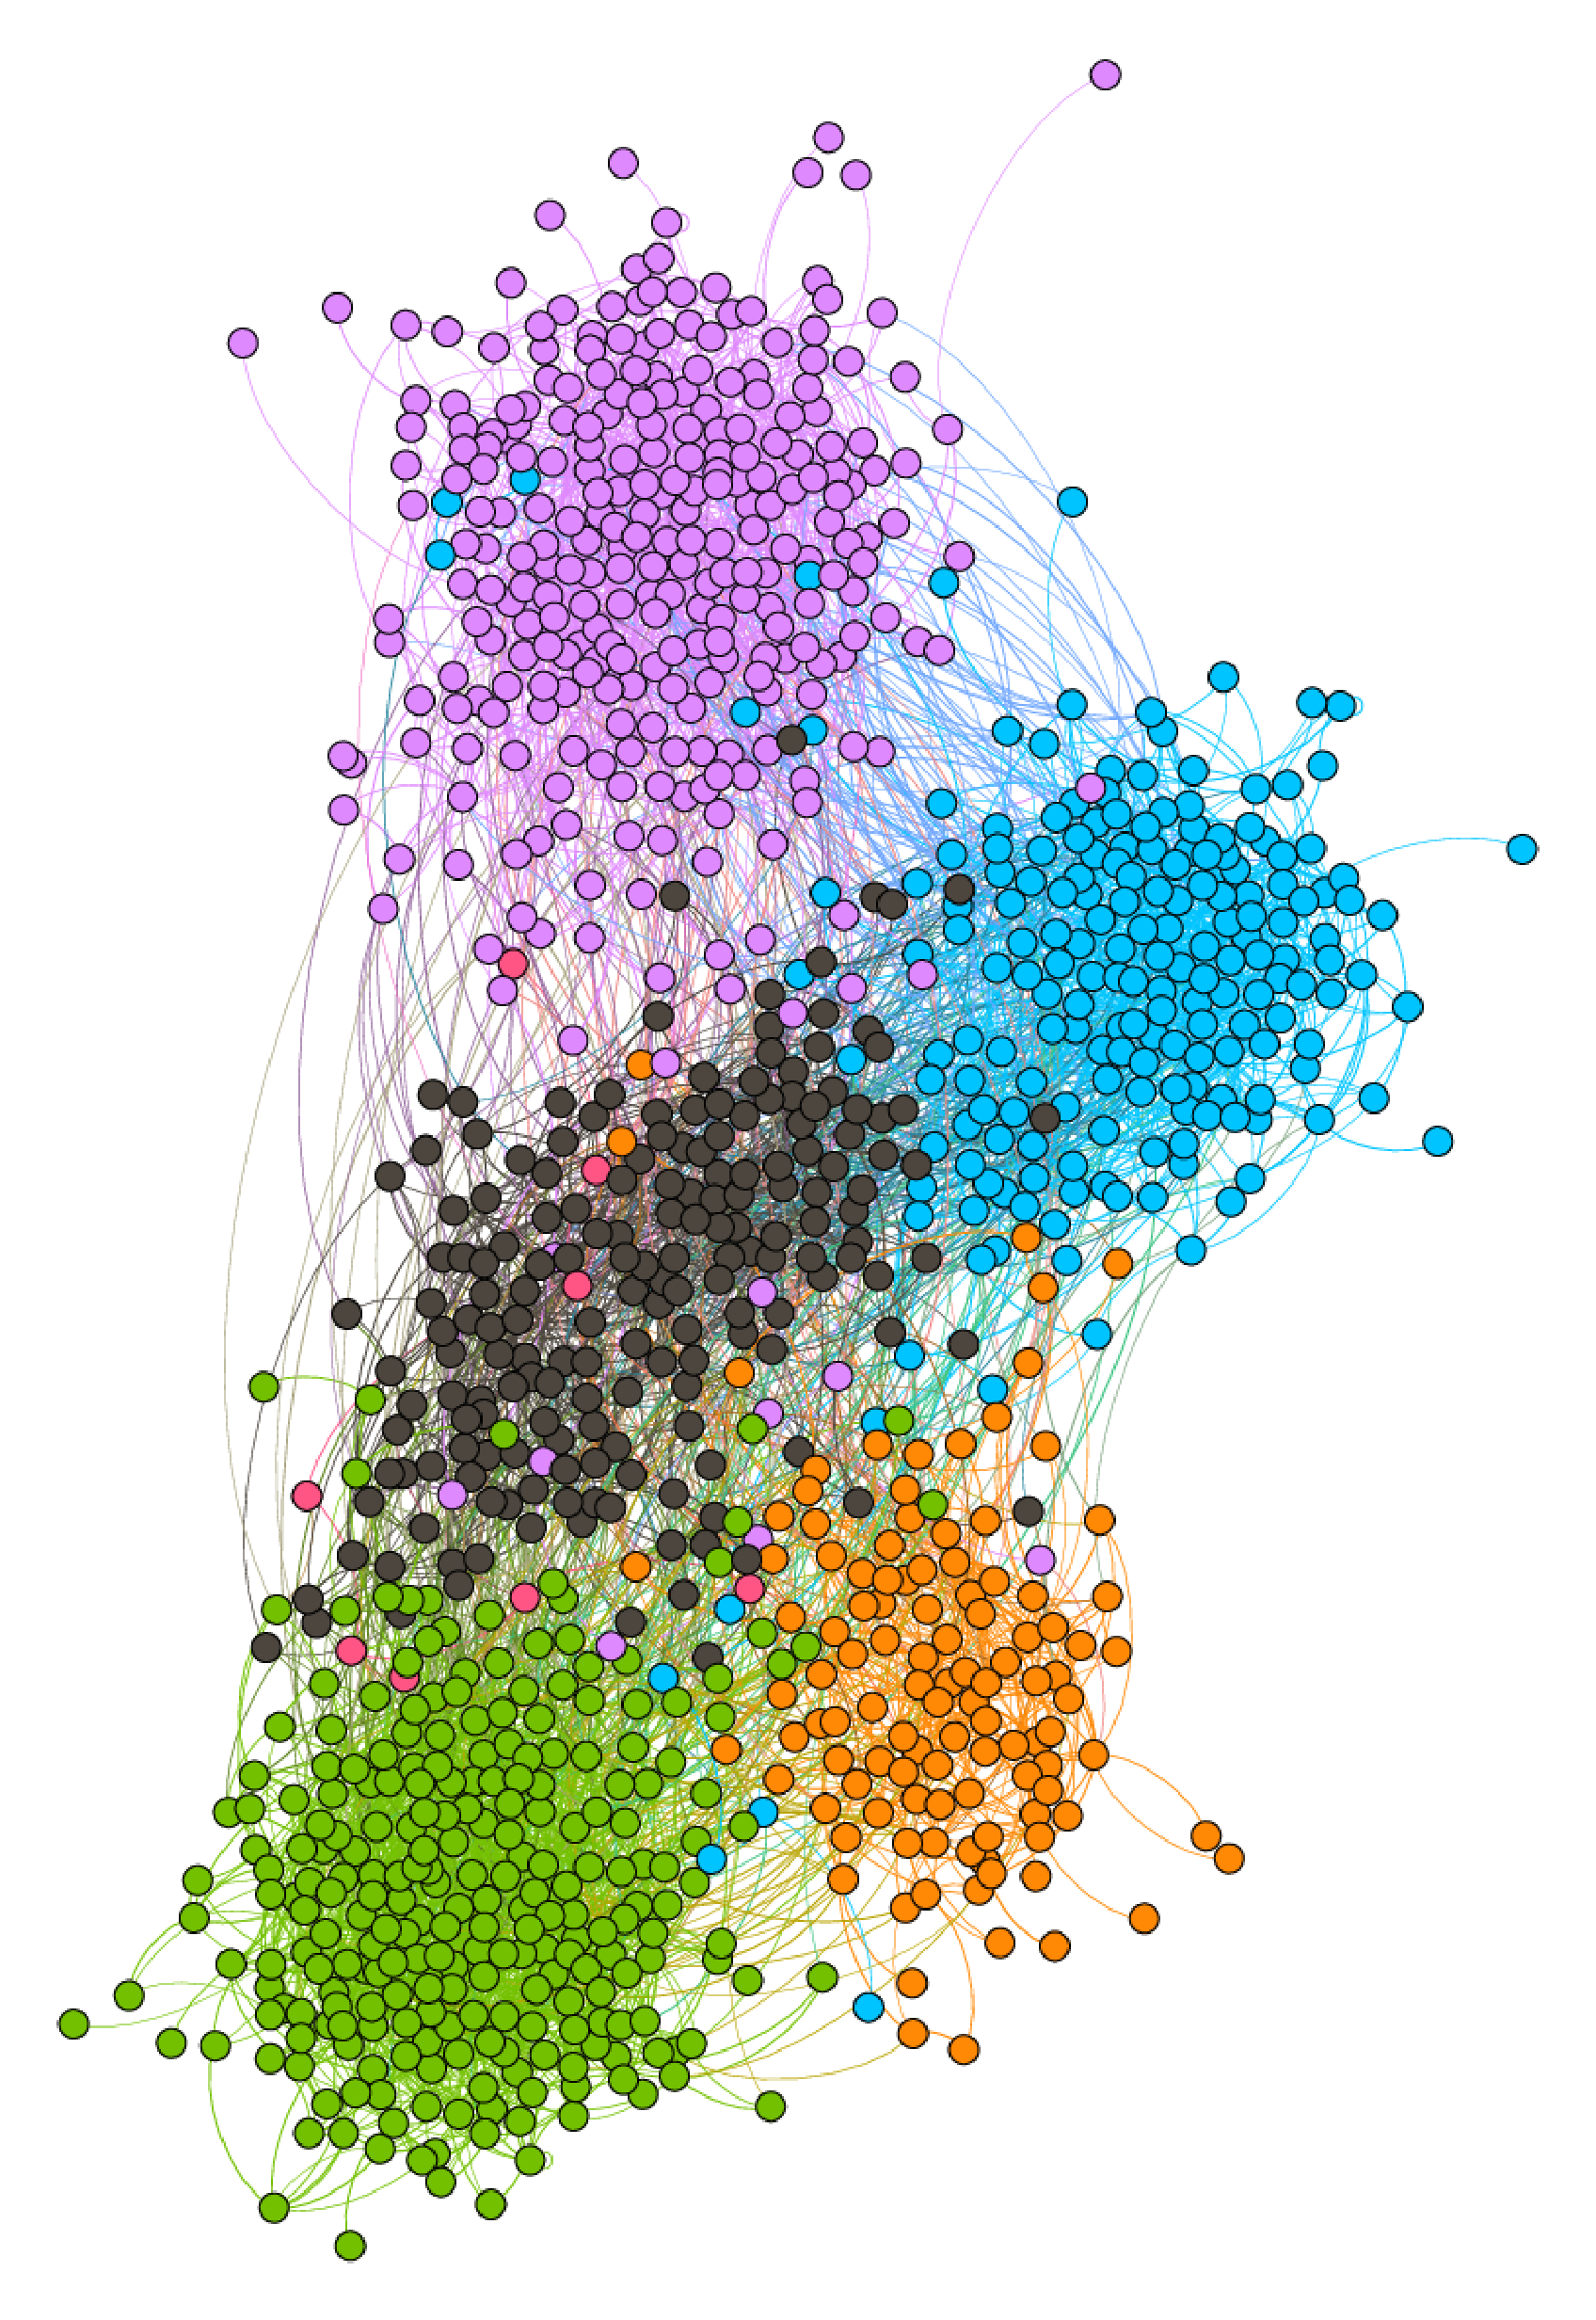
\includegraphics[width=\textwidth]{img/dim5_mod.pdf}
    \caption{bubble3news}
    \label{fig:bubble5mod}
  \end{subfigure}
  ~
  \begin{subfigure}[t]{0.35\textwidth}
    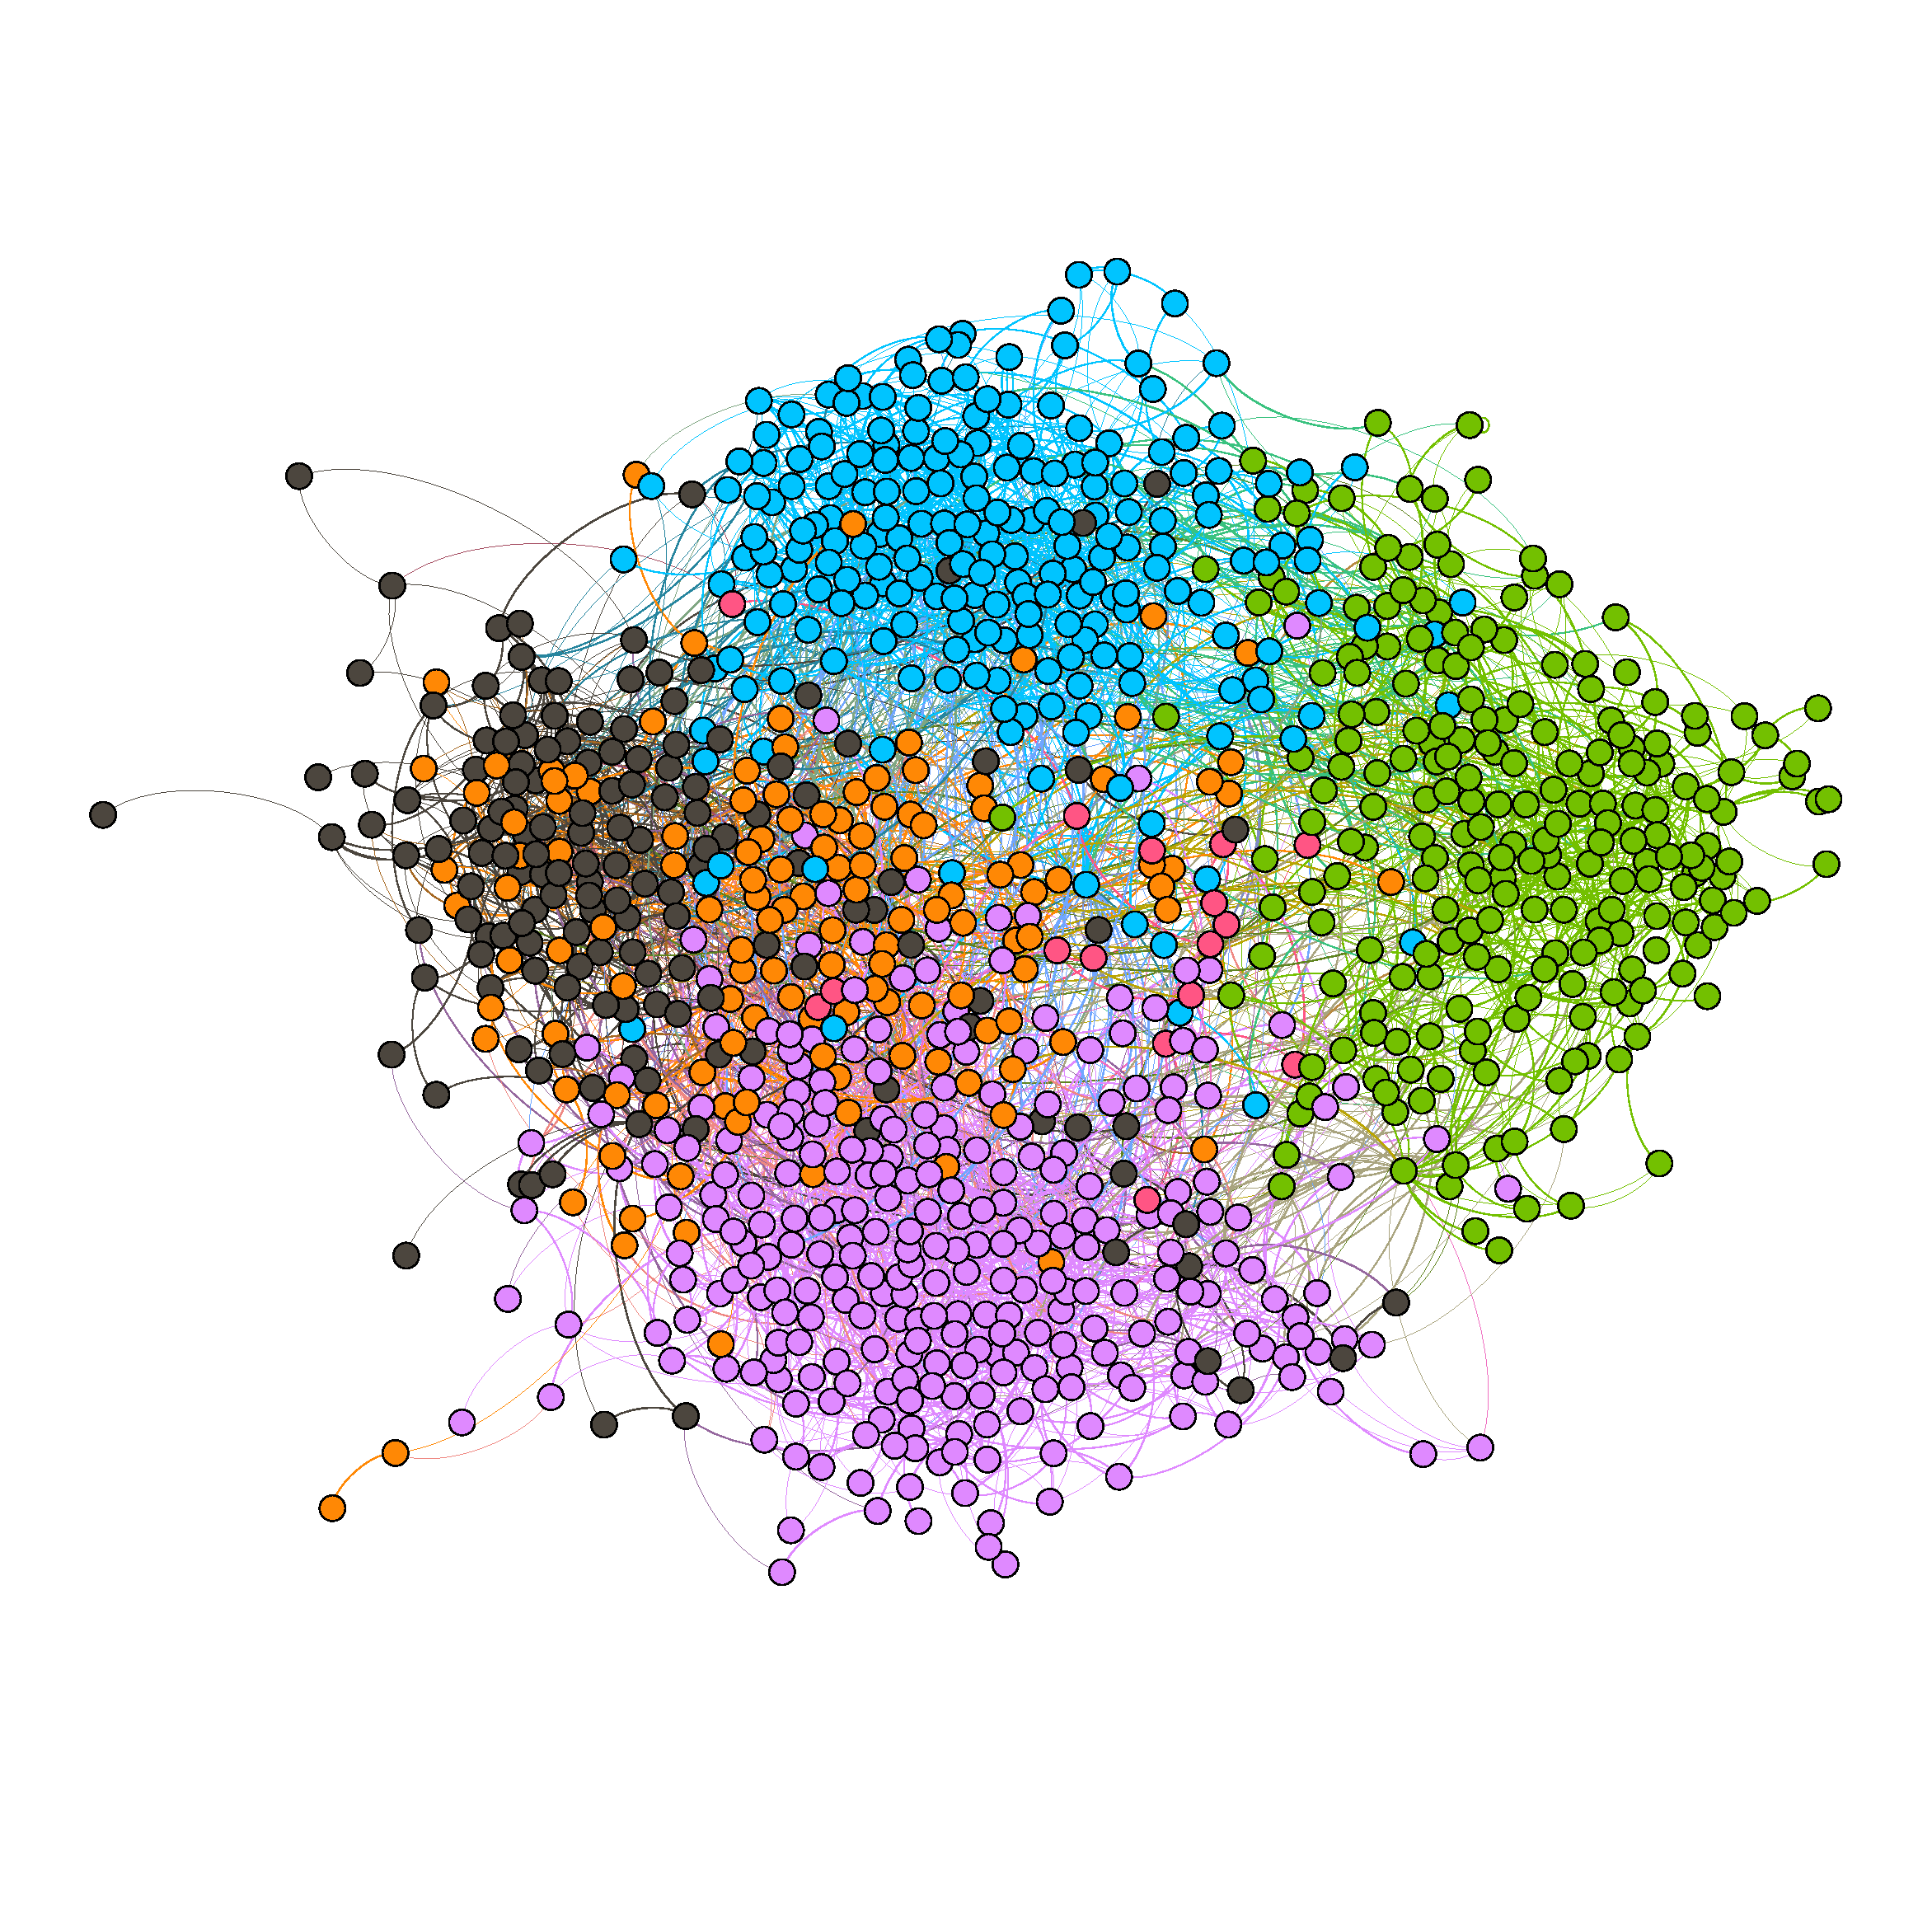
\includegraphics[width=\textwidth]{img/dim7_mod.pdf}
    \caption{bubble3news}
    \label{fig:bubble7mod}
  \end{subfigure}
  \\
  \begin{subfigure}[t]{0.25\textwidth}
    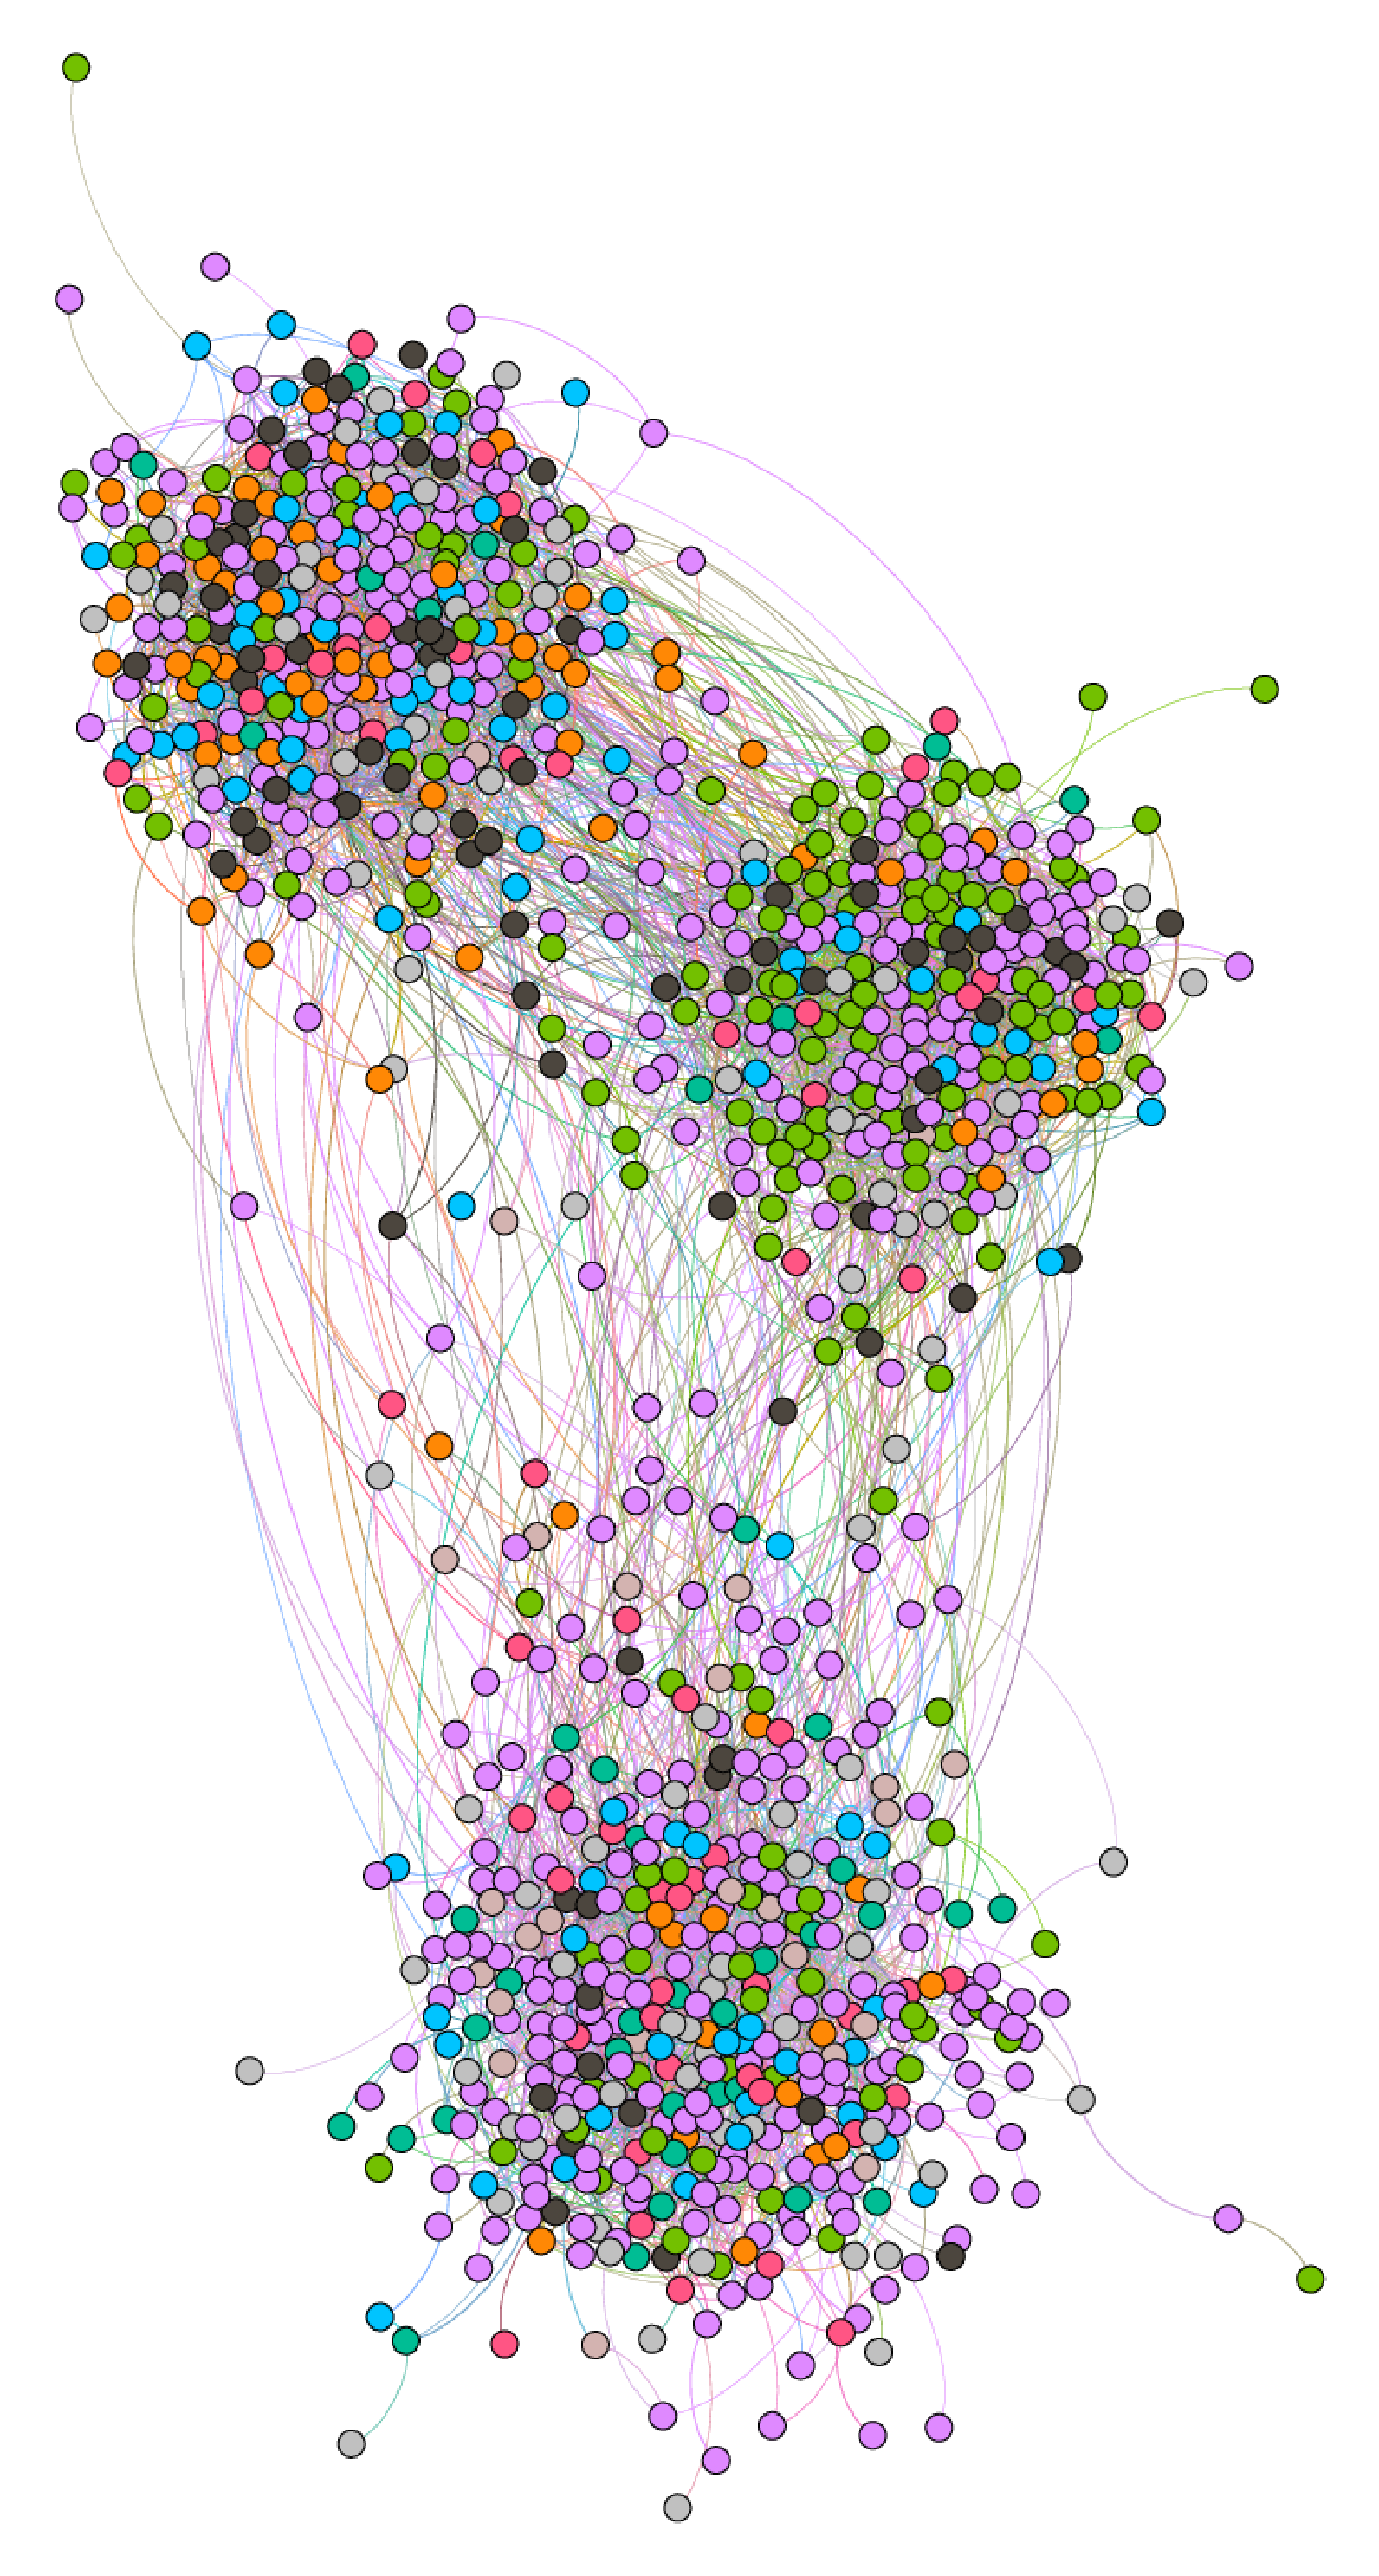
\includegraphics[width=\textwidth]{img/dim3_news.pdf}
    \caption{bubble3mod}
    \label{fig:bubble3news}
  \end{subfigure}
  ~
  \begin{subfigure}[t]{0.35\textwidth}
    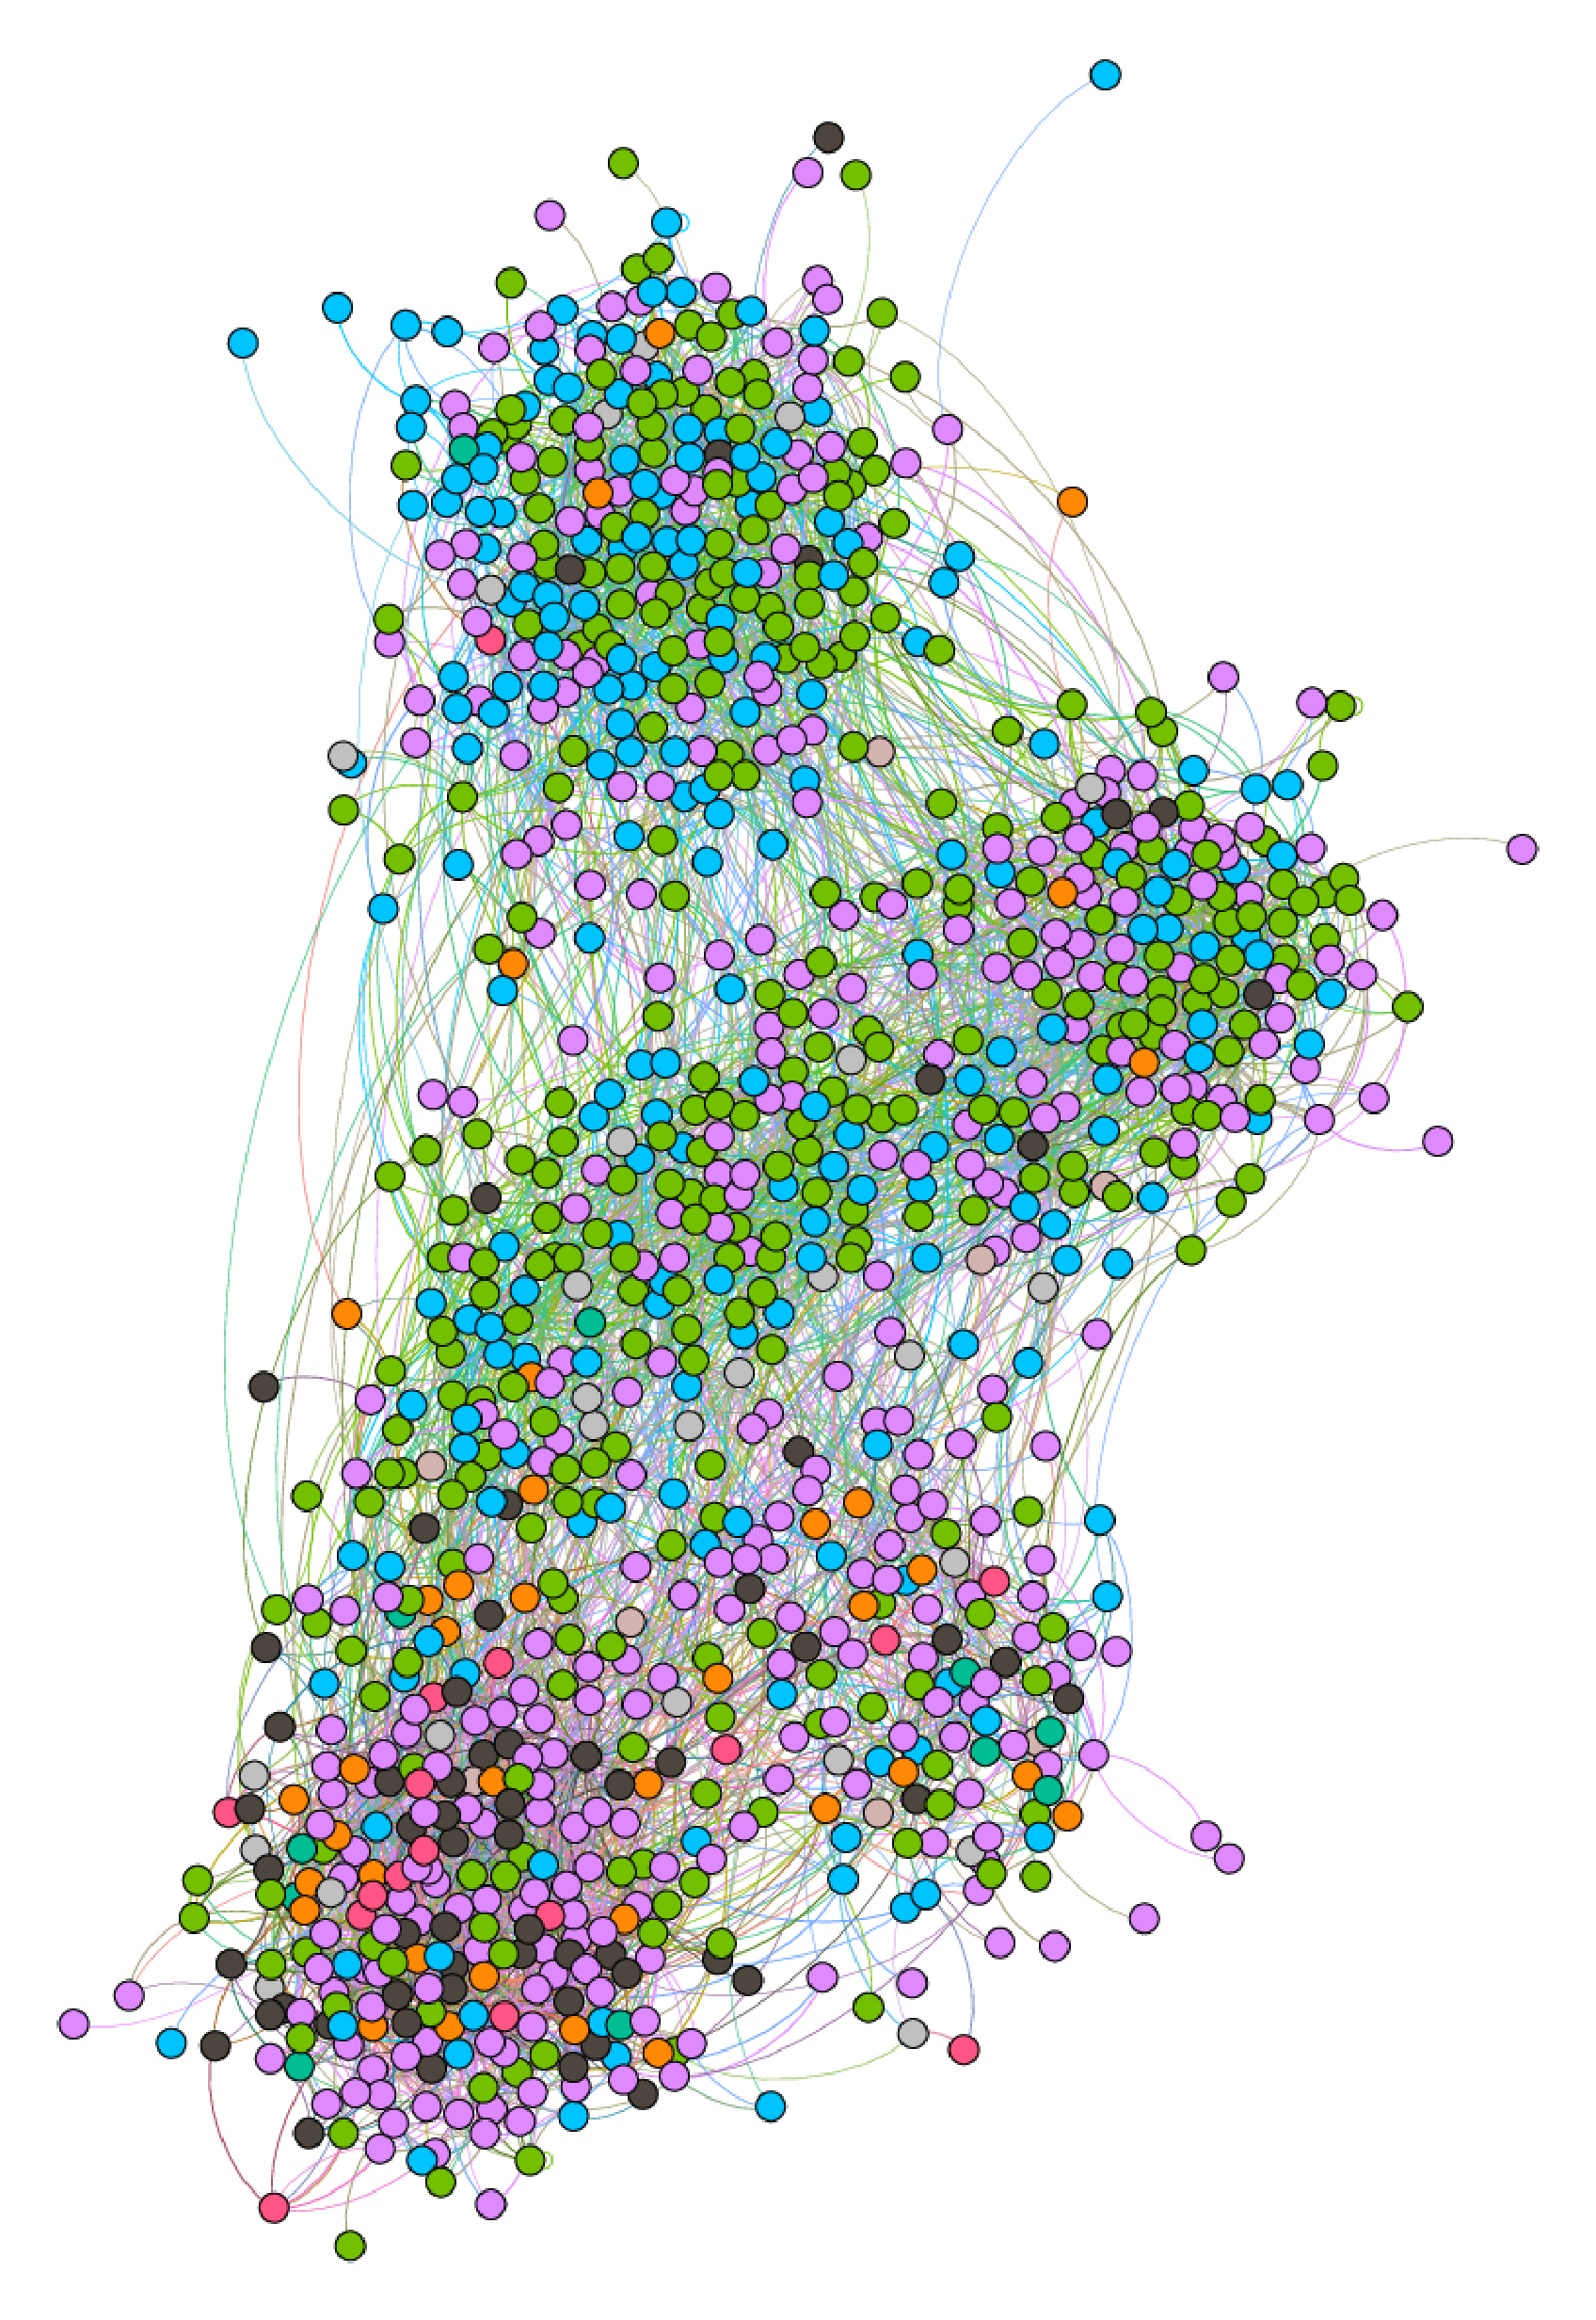
\includegraphics[width=\textwidth]{img/dim5_news.pdf}
    \caption{bubble3news}
    \label{fig:bubble5news}
  \end{subfigure}
  ~
  \begin{subfigure}[t]{0.35\textwidth}
    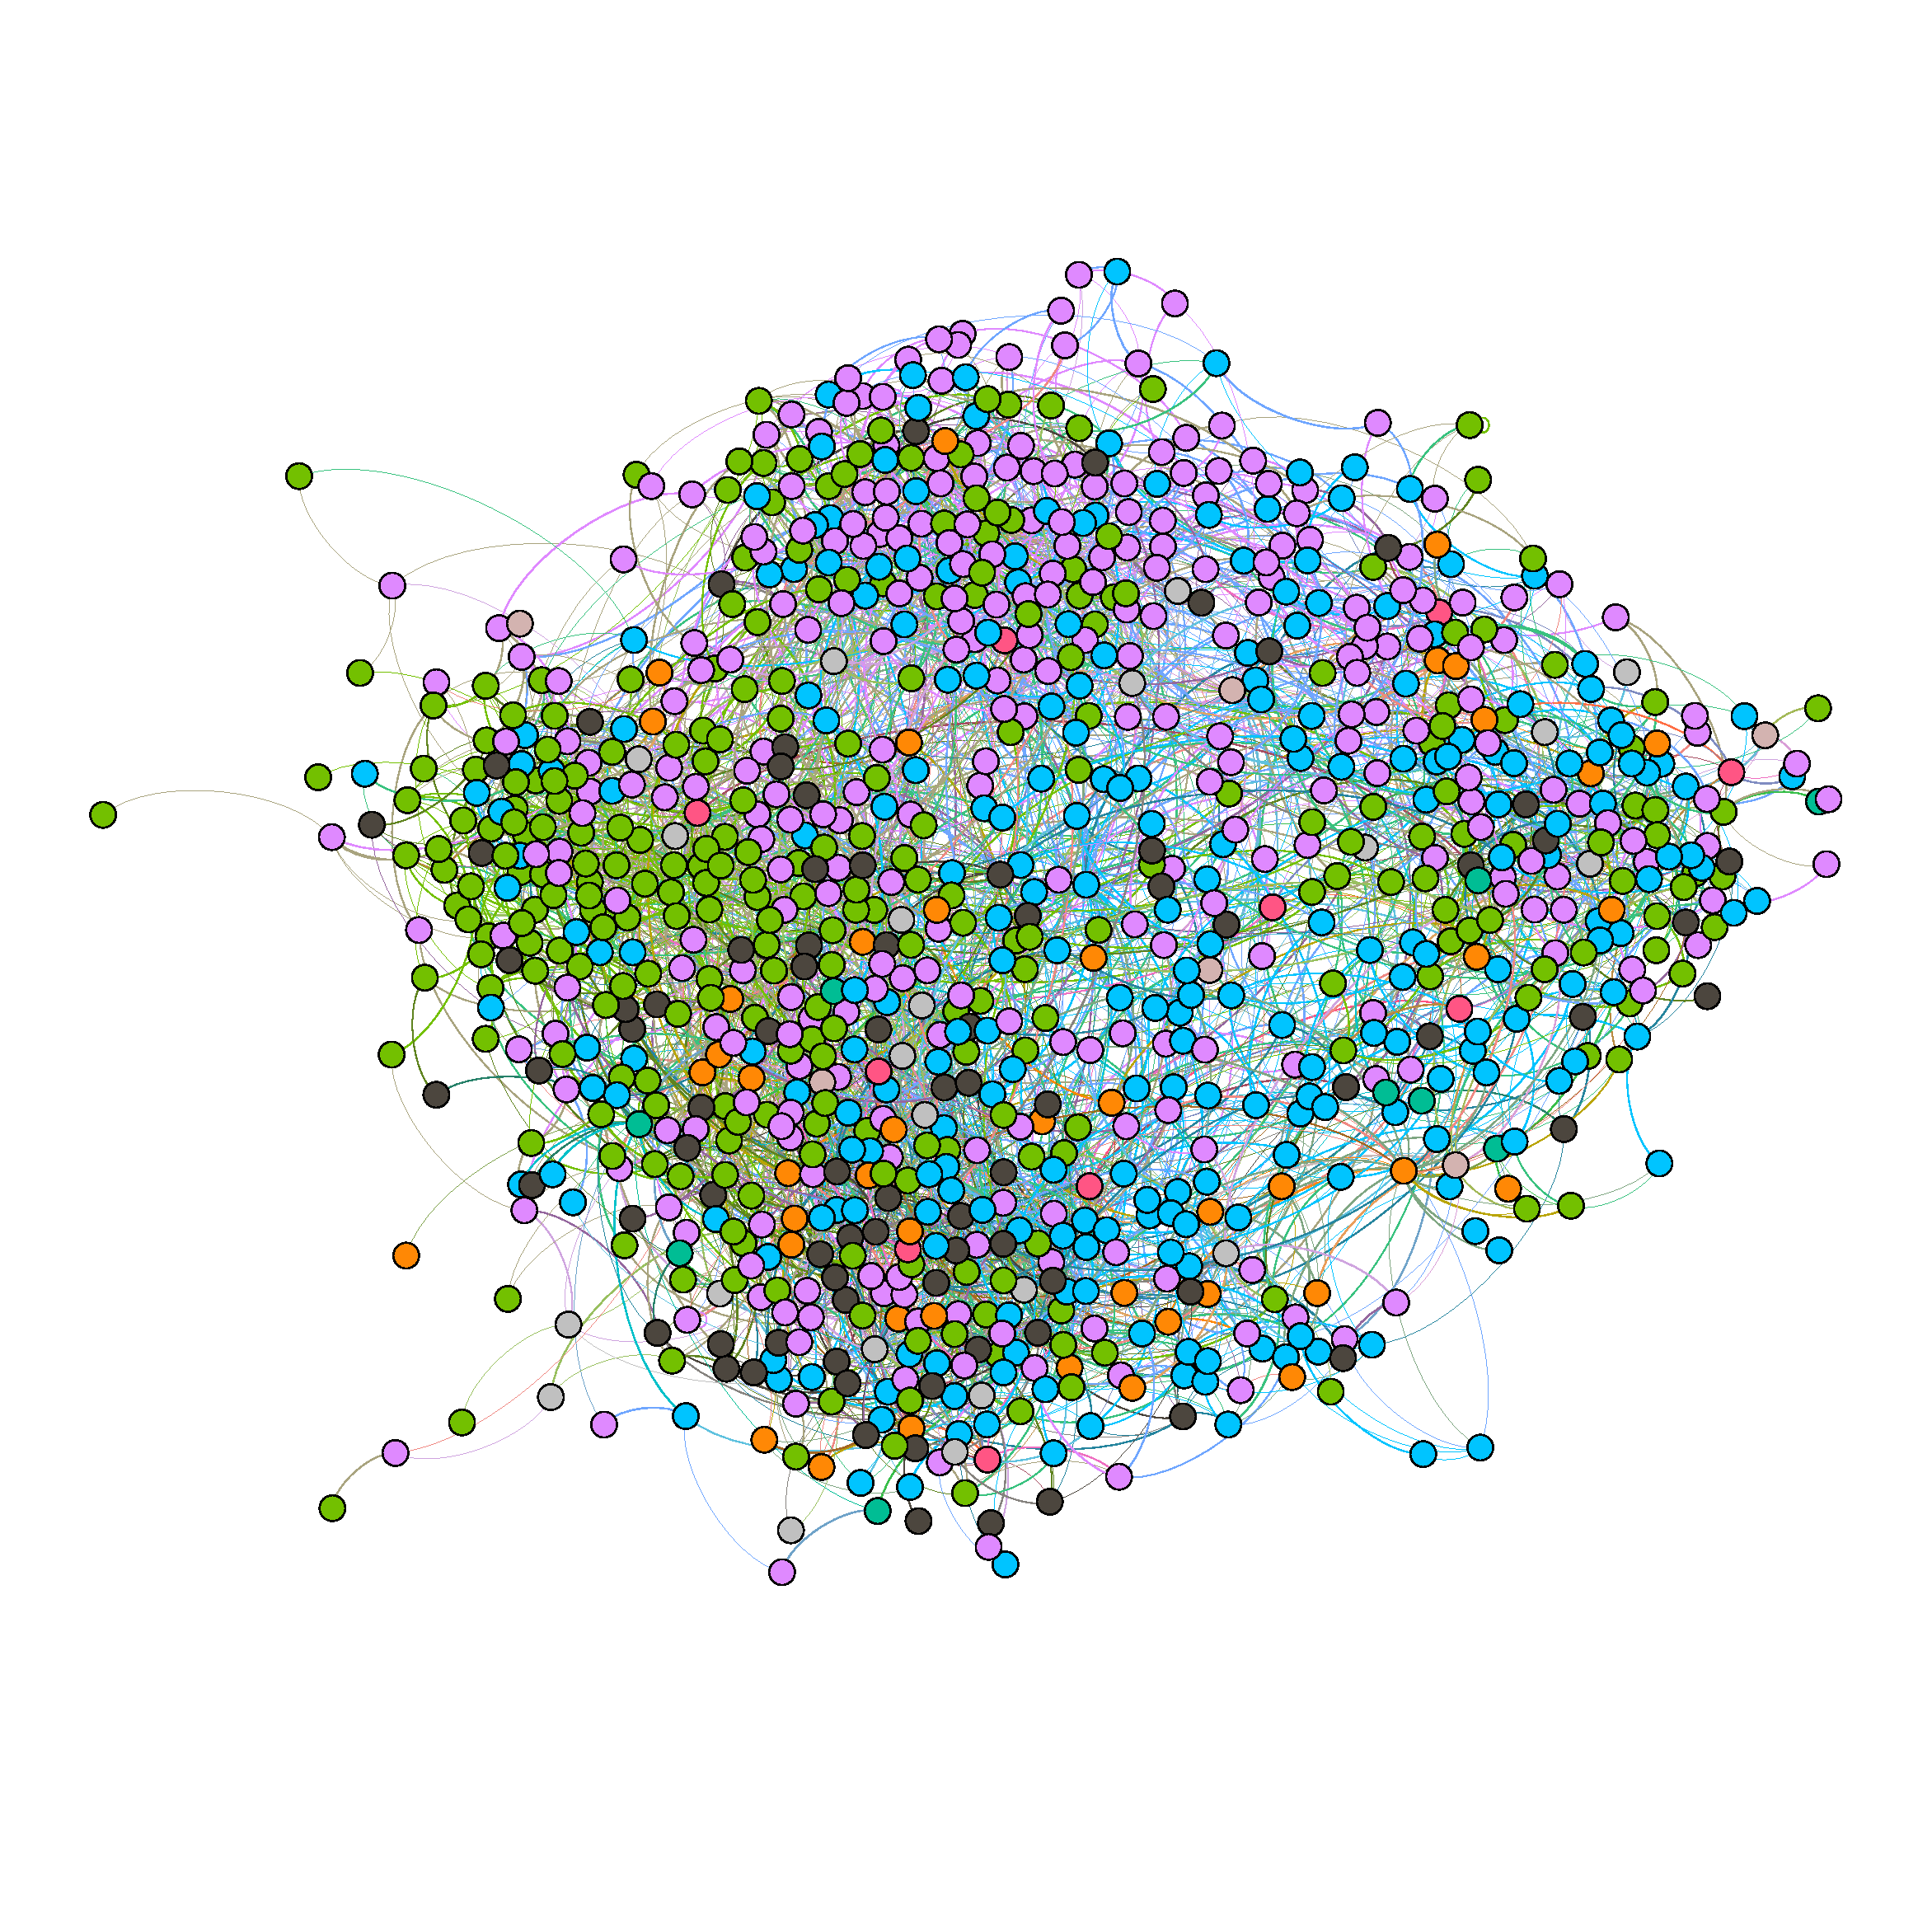
\includegraphics[width=\textwidth]{img/dim7_news.pdf}
    \caption{bubble3news}
    \label{fig:bubble7news}
  \end{subfigure}
  \caption[Network results: bubble chamber]{Simulations for 1000 users and 20 sources after 1000
    iterations. (\subref{fig:bubble3mod}), (\subref{fig:bubble5mod}) and
    (\subref{fig:bubble7mod}) highlights state vector.
    (\subref{fig:bubble3news}), (\subref{fig:bubble5news}) and
   (\subref{fig:bubble7news}) highlitghts different news.
  }
  \label{fig:test}
\end{figure}
